\documentclass[11pt,letterpaper]{article}

\addtolength{\oddsidemargin}{-.875in}
\addtolength{\evensidemargin}{-.875in}
\addtolength{\textwidth}{1.75in}

\addtolength{\topmargin}{-.875in}
\addtolength{\textheight}{1.75in}

\usepackage[utf8]{inputenc}
\usepackage{caption} % for table captions
\usepackage{amsmath} % for multi-line equations and piecewises
\DeclareMathOperator{\sign}{sign}
\usepackage{graphicx}
\usepackage{relsize}
\usepackage{xspace}
\usepackage{verbatim} % for block comments
\usepackage{subcaption} % for subfigures
\usepackage{enumitem} % for a) b) c) lists
\newcommand{\Cyclus}{\textsc{Cyclus}\xspace}%
\newcommand{\Cycamore}{\textsc{Cycamore}\xspace}%
\newcommand{\deploy}{\texttt{d3ploy}\xspace}%
\newcommand{\Deploy}{\texttt{D3ploy}\xspace}%
\usepackage{tabularx}
\usepackage{color}
\usepackage{multirow}
\usepackage{float} 
\usepackage[acronym,toc]{glossaries}
%\include{acros}
\definecolor{bg}{rgb}{0.95,0.95,0.95}
\newcolumntype{b}{X}
\newcolumntype{f}{>{\hsize=.15\hsize}X}
\newcolumntype{s}{>{\hsize=.5\hsize}X}
\newcolumntype{m}{>{\hsize=.75\hsize}X}
\newcolumntype{r}{>{\hsize=1.1\hsize}X}
\usepackage{titling}
\usepackage[hang,flushmargin]{footmisc}
\renewcommand*\footnoterule{}
\usepackage{tikz}

\usetikzlibrary{shapes.geometric,arrows}
\tikzstyle{process} = [rectangle, rounded corners, 
minimum width=1cm, minimum height=1cm,text centered, draw=black, 
fill=blue!30]
\tikzstyle{arrow} = [thick,->,>=stealth]

\graphicspath{}
% \title{MHTGR350}
%\author{Roberto E. Fairhurst Agosta}

\begin{document}
%	\begin{titlepage}
%		\maketitle
%		\thispagestyle{empty}
%	\end{titlepage}

\section{Introduction}

In 2013, the IAEA launched the Coordinated Research Project (CRP) on Uncertainty Analysis in Modeling (UAM) to study uncertainty propagation in the High Temperature Gas-cooled Reactor (HTGR) analysis chain.

HTGR reactors require core simulation techniques not typically utilized in Light Water Reactor (LWR) analysis due to several unique features, such as double heterogeneous fuel design including tristructural isotropic (TRISO) fuel particles, large graphite quantities, and high operational temperatures.

\cite{bostelmann_criticality_2016}.

A major challenge for neutronics modeling is the double heterogenity present in \glspl{HTGR}.

The issue of double heterogeneity arises from the introduction of the TRISO fuel particles into the reactor design.
These TRISO particles form the first level of heterogeneity, as they consist of four layers.
The second level of heterogeneity arises from the fuel elements themselves.
The TRISO particles are packed into fuel compacts, which are contained within fuel assemblies that are heterogeneous with the coolant, moderator, and reflector regions.

The computational time required to explicitly model individual TRISO particles in the reactor makes this approach time consuming, costly, and impractical for the majority of applications.
Applying a simple volume homogenization has proven to be insufficient for TRISO particle, due to the resonant self-shielding effect of the kernel and coated layers.

SERPENT is a continuous energy Monte Carlo reactor physics burnup calculation code, developed by VTT Technical Research Centre of Finland and distributed by RSICC in the United States.
SERPENT allows for the explicit modeling of TRISO fuel particles.

\cite{rahnema_whitepaper_2015}.

\section{CRP Exercise I-1}

Objective is to address the uncertainties due to double heterogeneity or self-shielding treatment.

Figure \ref{fig:compact} shows the MHTGR fuel compact unit cell.
This unit cell is derived from the fuel block hexagonal geometry, Figure \ref{fig:fuelblock}.

Exercise I-1a specifies a homogeneous fuel region.
Exercise I-1b specifies the TRISO fuel particles explicitly.

The problem uses a reflective boundary condition.
Two sub-cases: a Cold Zero Power (CZP) and Hot Full Power (HFP)
We will focus on the first one.

Differences to OECD MHTGR Benchmark.

	\begin{figure}[htbp!]
		\centering
		\begin{subfigure}[t]{0.4\textwidth}
			\centering
			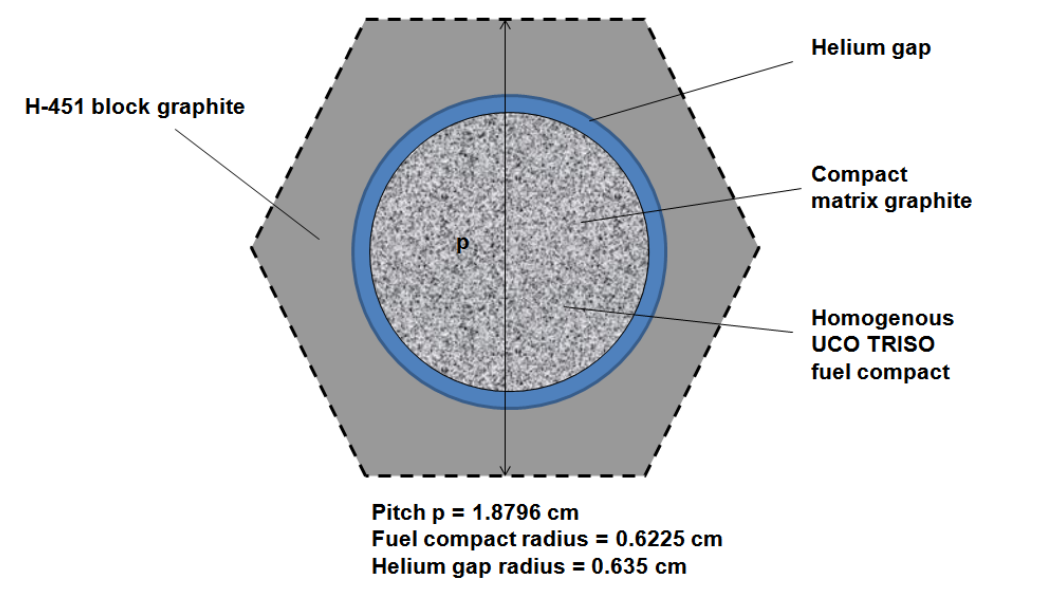
\includegraphics[width=\linewidth]{exerciseI-1-geo}
			\caption{MHTGR fuel compact unit cell for Exercise I-1.}
			\label{fig:compact}
		\end{subfigure}
		\begin{subfigure}[t]{0.4\textwidth}
			\centering
			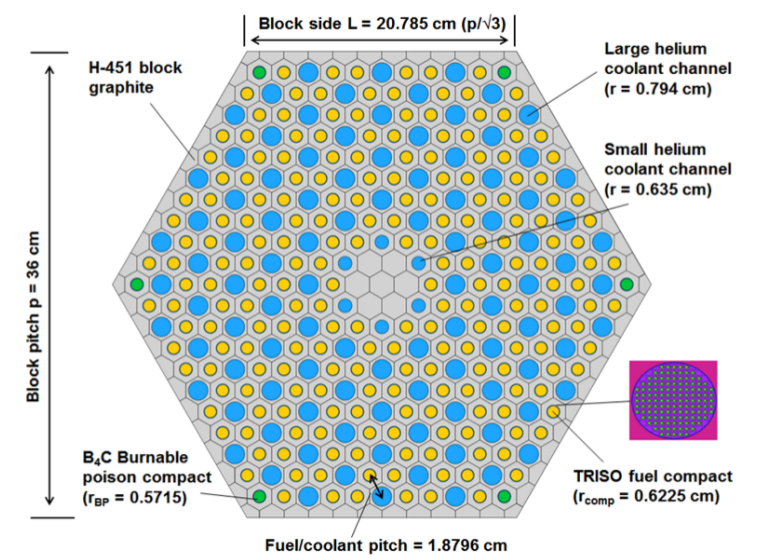
\includegraphics[width=\linewidth]{exerciseI-2-geo}
			\caption{MHTGR fuel block for Exercise I-2.}
			\label{fig:fuelblock}
		\end{subfigure}
		\hfill
		\caption{MHTGR fuel compact unit cell for Exercise I-1. Image reproduced from \cite{strydom_results_2015}.}
		\label{fig:fuel}
	\end{figure}

HFP:
ExerciseI-1a.
50000 neutrons/cycle, 500 active cycles, 50 inactive cycles.
3.11 min. MPI = 8, OMP = 8: 64 cores.
six_ff_keff = 1.19156 +/- 0.00021

% OMP: OpenMP threads = number of available processor cores.
% MPI: Amount of processes.

% Ex: 2 sockets (2 physical CPUs) with 12 cores (total 24 cores): OMP = 24.
% Ex: 2 Computers with 2 sockets and 12 cores/socket (total 48 cores): MPI = 2, OMP = 24.

ExerciseI-1b. 
50000 neutrons/cycle, 500 active cycles, 50 inactive cycles.
4.04 min. MPI = 8, OMP = 8: 64 cores.
six_ff_keff = 1.25411 +/- 0.00020

Although ExerciseI-1b runs a 30\% slower K$_{eff}$ changes considerably.

ExerciseI-1bE. 
50000 neutrons/cycle, 500 active cycles, 50 inactive cycles.
4.04 min. MPI = 8, OMP = 8: 64 cores.
six_ff_keff = 1.25411 +/- 0.00020

Reference result using (I don't know what version mine is):
42.7 min. OMP = 4.
six_ff_keff = 1.25303 +/- 0.00019

ENDFB7.0 1.24657 ± 0.00013
ENDFB7.1 1.24525 ± 0.00014

\section{CRP Exercise I-2}

Exercise I-2a: fresh single block, Figure \ref{fig:fuelblock}.
Exercise I-2b: depleted block, similar to Figure \ref{fig:fuelblock} but without the LBP compacts.

Exercise I-2a:
200000 neutrons/cycle, 500 active cycles, 50 inactive cycles.
1.28 h. MPI = 8, OMP = 16: 128 cores.
six_ff_keff = 1.06523 +/- 0.00011

\section{OECD Exercise I}

oecd-exI-1b1: Figure \ref{fig:compact}.
same material composition as OECD MHTGR 350 (the one I calculated)
six_ff_keff = 1.25205 +/- 0.00019
4 min MPI = 8, OMP = 16

oecd-exI-1b2:
same material composition as CRP
six_ff_keff = 1.24348 +/- 0.00020
4.01 min MPI = 8, OMP = 16

oecd-exI-1b3:
same material composition as OECD MHTGR 350 - Phase III
six_ff_keff = 1.24872 +/- 0.00020
4.01 min MPI = 8, OMP = 16

\begin{figure}[htbp!]
	\centering
	\includegraphics[height=5cm]{oecd-exI-1b1.png}
	\caption{Compact.}
	\label{fig:compact}
\end{figure}

oecd-exI-2a: Figure \ref{fig:assembly}.
same material composition as OECD MHTGR 350 - Phase III
six_ff_keff = 1.07006 +/- 0.00011
1.29 h MPI = 8, OMP = 16

\begin{figure}[htbp!]
	\centering
	\includegraphics[height=5cm]{oecd-exI-2a.png}
	\caption{Fuel Assembly.}
	\label{fig:assembly}
\end{figure}

\section{OECD Standard-column}

Figure \ref{fig:stcol}.
same material composition as OECD MHTGR 350 - Phase III
six_ff_keff = 1.07201 +/- 0.00007
4.24 h MPI = 8, OMP = 16

\begin{figure}[htbp!]
	\centering
	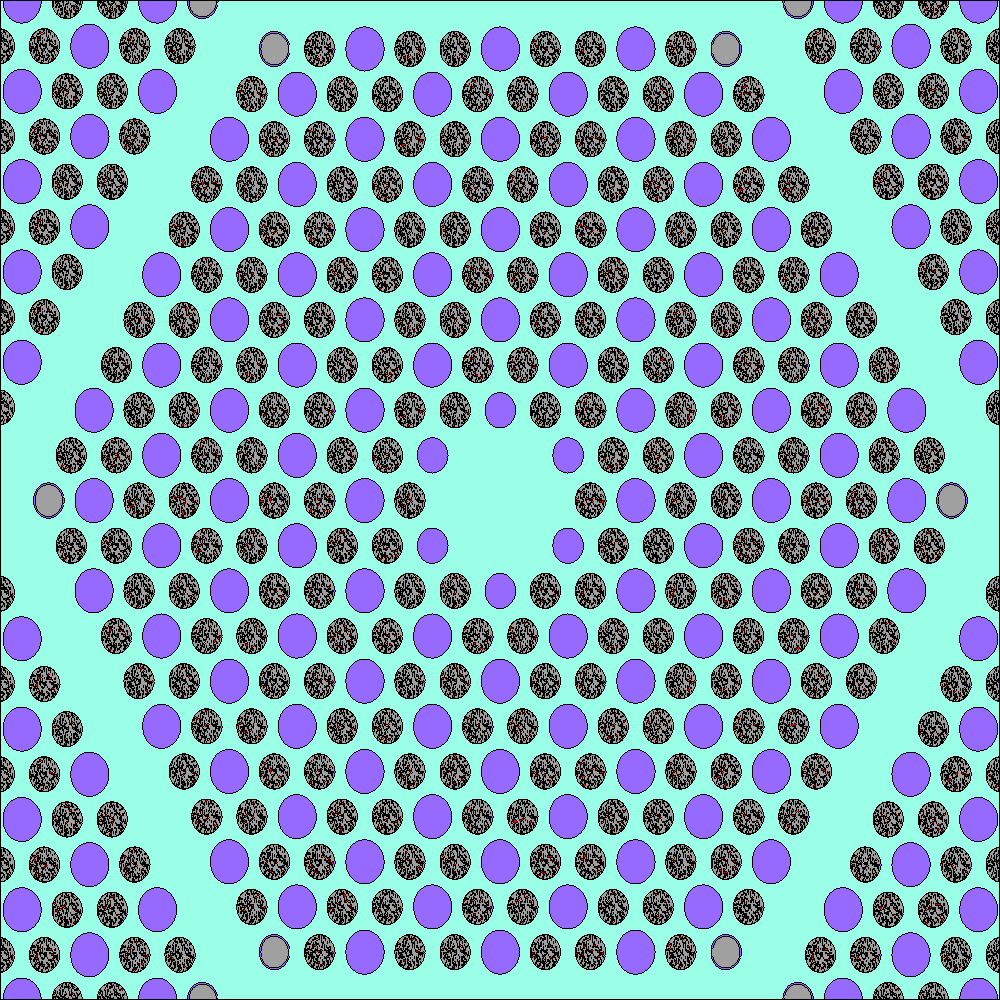
\includegraphics[height=5cm]{oecd-standard-column_geom1.png}
	\caption{Standard column.}
	\label{fig:stcol}
\end{figure}

\section{OECD Fullcore}

Figure \ref{fig:fullcore}.
same material composition as OECD MHTGR 350 - Phase III
six_ff_keff = 1.06284 +/- 0.00006
10.6 h MPI = 8, OMP = 16

\begin{figure}[htbp!]
	\centering
	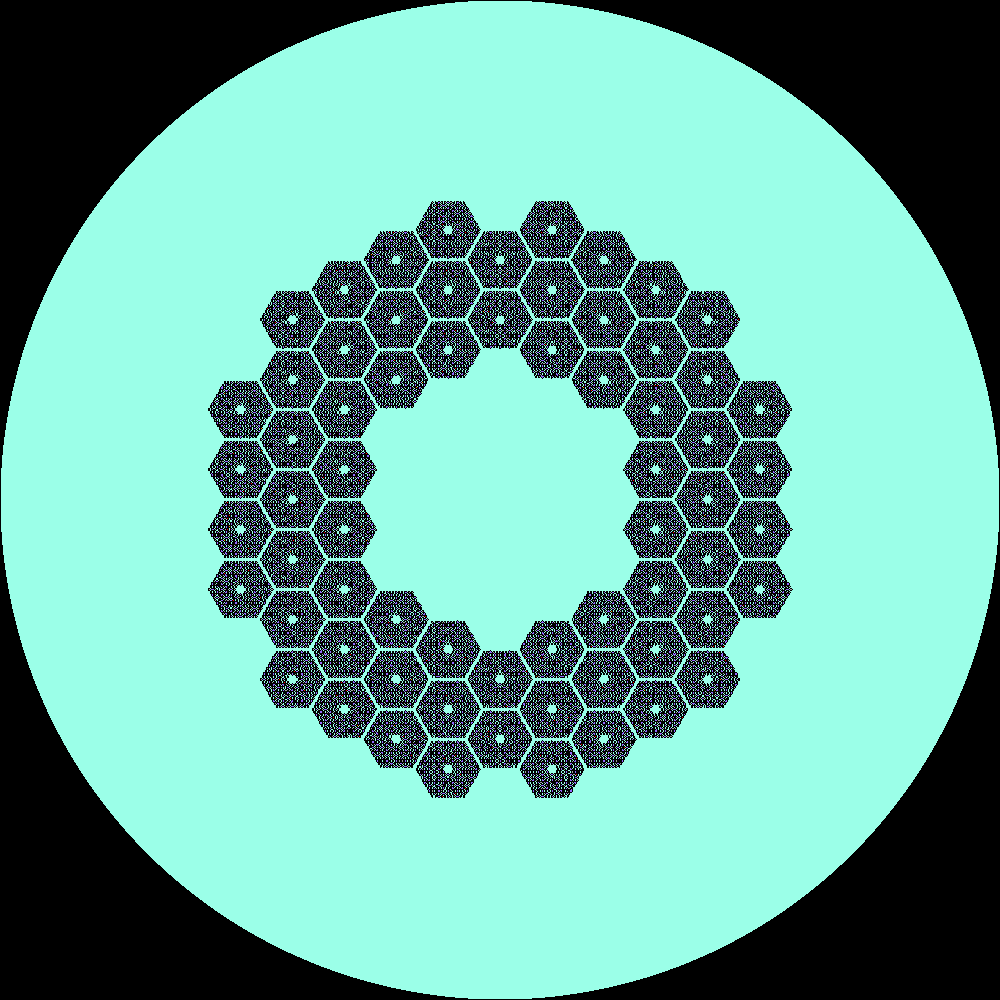
\includegraphics[height=5cm]{oecd-fullcore_geom1.png}
	\caption{Full core.}
	\label{fig:fullcore}
\end{figure}

\pagebreak
\bibliographystyle{plain}
\bibliography{bibliography}

\end{document}

	% \begin{table}[]
	% 	\centering
	%     \caption{TRISO and Fuel Compact Characteristics.}
	%     \label{tab:compact}
	% 	\begin{tabular}{l|l}
	% 	\hline
	% 	Characteristic                   & Value                \\ \hline
	% 	Fuel                             & UC$_{0.5}$O$_{1.5}$  \\
	% 	Enrichment (average)             & 15.5 wt\%            \\
	% 	Kernel radius                    & 0.02125 cm           \\
	% 	Buffer radius                    & 0.03125 cm           \\
	% 	IPyC radius                      & 0.03475 cm           \\
	% 	SiC radius                       & 0.03825 cm           \\
	% 	OPyC radius                      & 0.04225 cm           \\
	%  	Kernel density                   & 10.5 g/cm$^3$        \\
	% 	Buffer density                   & 1.0 g/cm$^3$         \\
	% 	IPyC density                     & 1.9 g/cm$^3$         \\
	% 	SiC density                      & 3.2 g/cm$^3$         \\
	% 	OPyC density                     & 1.9 g/cm$^3$         \\
	% 	Packing Fraction (average)       & 0.35                 \\
	% 	Compact radius                   & 0.6223 cm            \\
	% 	Compact Gap radius               & 0.635 cm             \\
	% 	Compact length                   & 4.928 cm             \\ 
	%   Helium density           		 & 4.19 kg/m$^3$        \\
	%   Block graphite density           & 1.85 g/cm$^3$        \\ \hline

	% 	\end{tabular}
	% \end{table}

	% \begin{figure}[htbp!]
	% 	\centering
	% 	\begin{subfigure}[t]{0.4\textwidth}
	% 		\centering
	% 		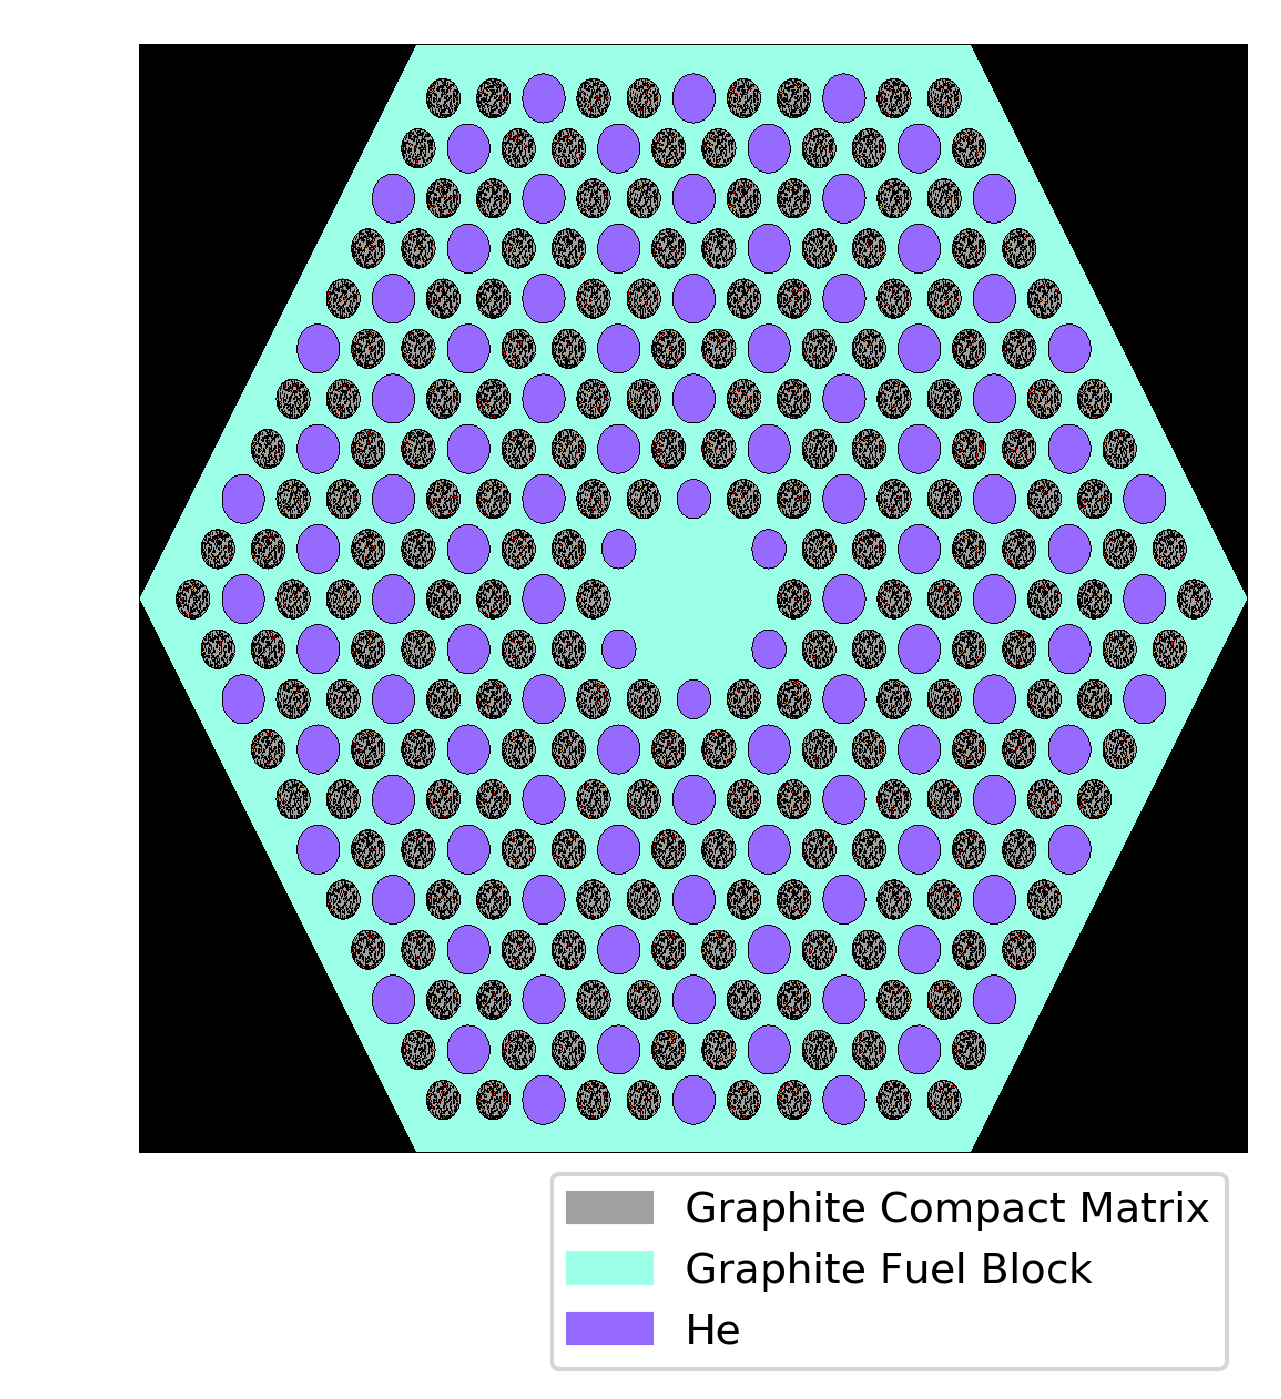
\includegraphics[width=\linewidth]{figures/standard.png}
	% 		\caption{XY-plane.}
	% 	\end{subfigure}
	% 	\begin{subfigure}[t]{0.4\textwidth}
	% 		\centering
	% 		\includegraphics[width=\linewidth]{figures/standard-column.png}
	% 		\caption{YZ-plane.}
	% 	\end{subfigure}
	% 	\hfill
	% 	\caption{Plot of \textit{standard-column}.}
	% 	\label{fig:standardcolumn}
	% \end{figure}

	% \begin{figure}[htbp!]
	% 	\centering
	% 	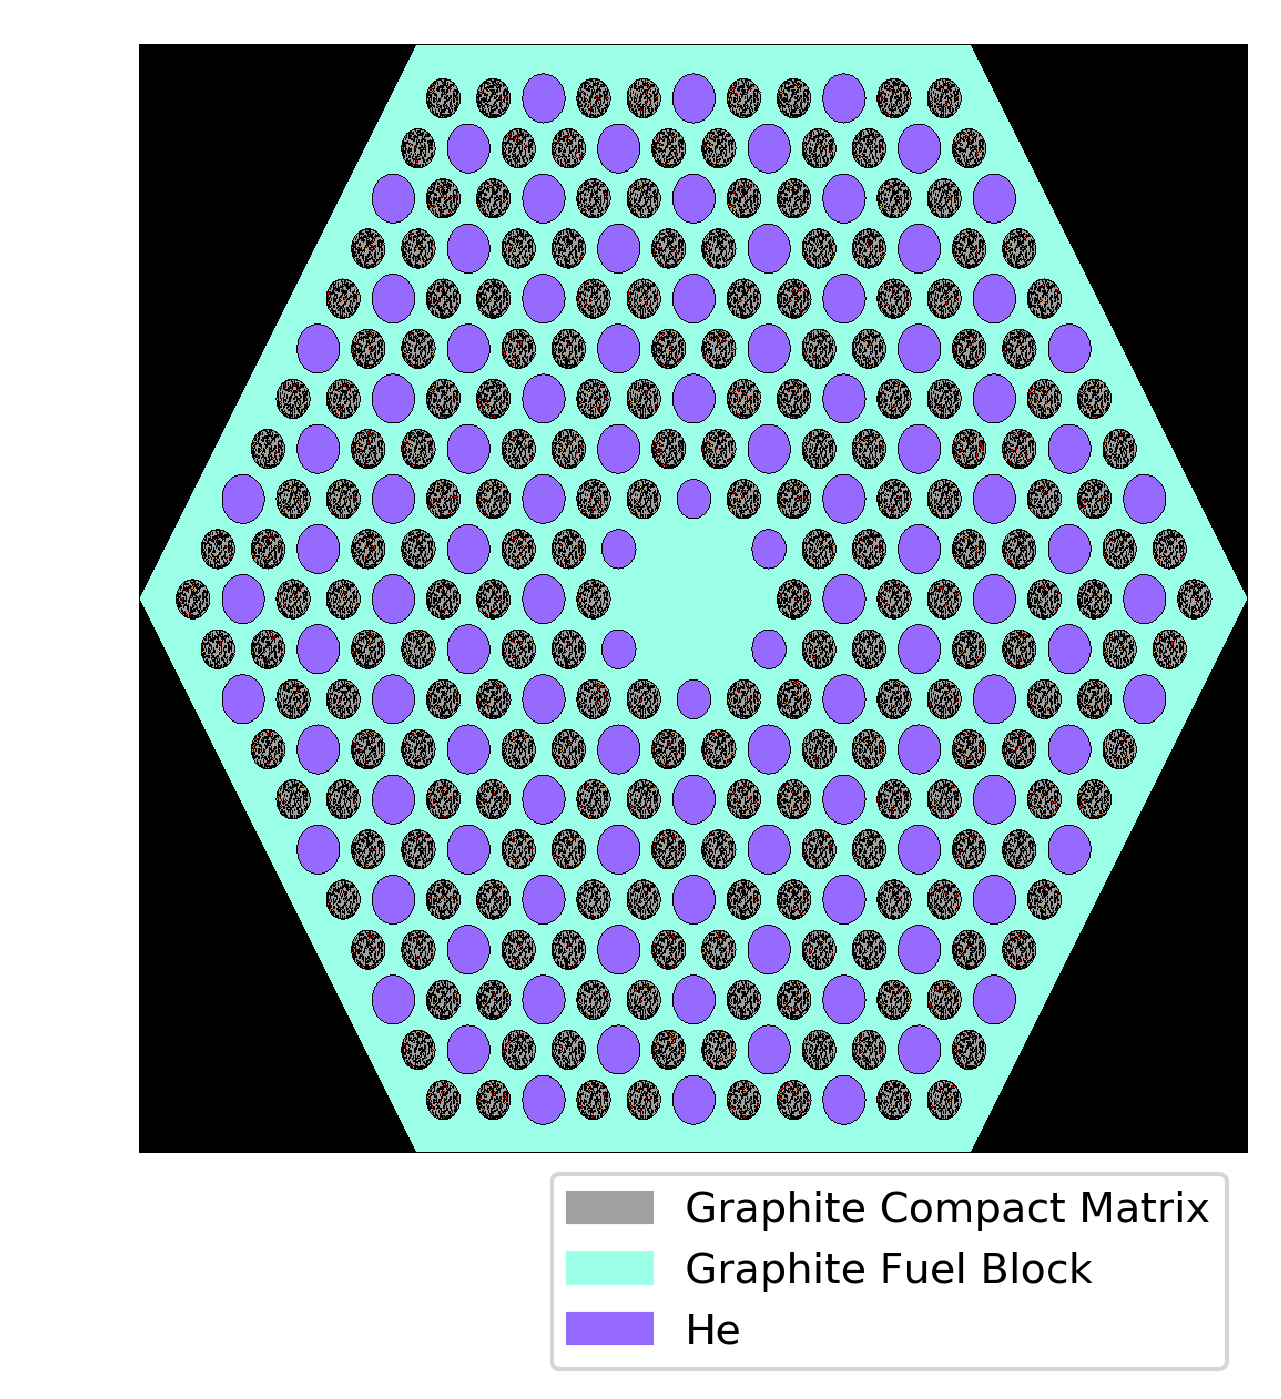
\includegraphics[height=5cm]{figures/standard.png}
	% 	\caption{Standard fuel assembly model.}
	% 	\label{fig:standard}
	% \end{figure}